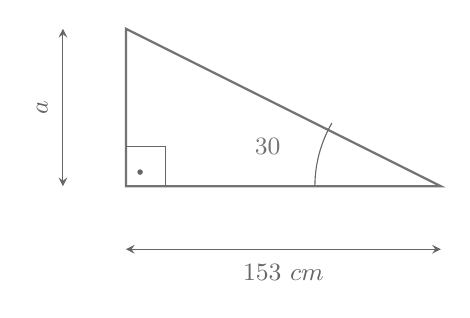
\begin{tikzpicture}[
    scale=2,
    cota/.style={<->, >=stealth, thin, gray!80!black},
    chamada/.style={gray!60, thin, dashed}
]
    % 1. Coordenadas dos vértices (Triângulo Retângulo 3-4-5)
    \coordinate (A) at (0,0); % Canto do ângulo reto
    \coordinate (B) at (2,0); % Canto inferior direito
    \coordinate (C) at (0,1); % Canto superior esquerdo

    % 2. Desenho do Triângulo
    \draw[thick, gray!90!black] (A) -- (B) -- (C) -- cycle;

    % 3. Símbolo de Ângulo Reto (90°)
    \draw[thin, gray!80!black] (0, 0.25) -- (0.25, 0.25) -- (0.25, 0);
    \fill[gray!80!black] (0.09, 0.09) circle (0.5pt);

    % 4. Indicação do Ângulo Theta em B
    \draw[thin, gray!80!black] (1.2, 0) arc (180:149.9:0.8);
    \node[font=\small, gray!90!black] at (0.9, 0.25) {$30$};

    % --- COTAS DE TAMANHO ---
    % Base (Cateto b)
    \def\offsetH{0.4}
    %\draw[chamada] (A) -- (0, -\offsetH - 0.05);
    %\draw[chamada] (B) -- (4, -\offsetH - 0.05);
    \draw[cota] (0, -\offsetH) -- (2, -\offsetH)
        node[midway, below=2pt, font=\small] {$153 \  \text{ cm}$};

    % Altura (Cateto a)
    \def\offsetV{0.4}
    %\draw[chamada] (A) -- (-\offsetV - 0.05, 0);
    %\draw[chamada] (C) -- (-\offsetV - 0.05, 3);
    \draw[cota] (-\offsetV, 0) -- (-\offsetV, 1)
        node[midway, left=2pt, font=\small, rotate=90, anchor=south] {$a$};

    % Hipotenusa (c) - Cota inclinada e paralela
    %\def\offsetHip{0.4}
    %\coordinate (B_cota) at ($(B) + (36.87:\offsetHip)$);
    %\coordinate (C_cota) at ($(C) + (36.87:\offsetHip)$);

    %\draw[chamada] (B) -- ($(B) + (36.87:\offsetHip + 0.05)$);
    %\draw[chamada] (C) -- ($(C) + (36.87:\offsetHip + 0.05)$);
    %\draw[cota] (B_cota) -- (C_cota)
        %node[midway, above right=-1pt, font=\small, rotate=-36.87] {$c = 5\text{ cm}$};

\end{tikzpicture}